\documentclass[a4paper,11pt, oneside]{report}

% Package import
\usepackage[a4paper,inner=3.5cm,outer=2.5cm]{geometry}
\usepackage[english,american]{babel}
\usepackage{fancyhdr}
\usepackage{latexsym}
\usepackage[T1]{fontenc}
\usepackage[utf8]{inputenc}
\usepackage{graphicx}
\usepackage{hyperref}
\usepackage{tabularx}
\usepackage{etoolbox}
\usepackage{fancyhdr}
\usepackage{amsthm}
\usepackage{mathtools}
\usepackage[xindy]{glossaries}
\usepackage{lastpage}
\usepackage{float}
\usepackage{fancyhdr}

\theoremstyle{definition}
\newtheorem{exmp}{Beispiel}[subsection]

\makeglossaries

\setcounter{secnumdepth}{2}
\setcounter{tocdepth}{1}


% clear default
\fancyhead{}
\fancyfoot{}

\usepackage{fancyhdr}
\pagestyle{fancy}
\fancyhf{}
\renewcommand{\headrulewidth}{0pt} % optional
\fancyfoot[L]{Chapter: \nouppercase{\leftmark}}
\fancyfoot[R]{\thepage/\pageref{LastPage}}

% Redefine the plain page style, Chpater page
\fancypagestyle{plain}{%
  \fancyhf{}
  \renewcommand{\headrulewidth}{0pt} % optional
  \fancyfoot[R]{\thepage/\pageref{LastPage}}
}

\renewcommand{\chaptermark}[1]{\markboth{\MakeUppercase{#1}}{}}


% URL Line breaks
\makeatletter
\g@addto@macro{\UrlBreaks}{\UrlOrds}
\makeatother

\begin{document}


\pagestyle{empty} %Keine Kopf-/Fusszeilen auf den ersten Seiten.
\begin{titlepage}
\begin{center}

% Oberer Teil der Titelseite:

\includegraphics[width=0.08\textwidth]{img/bfh_logo.png}\\[1cm]    
\textsc{\LARGE Bern University of Applied Sciences}\\[1.5cm]
\textsc{\Large Informatics Seminar}\\[0.5cm]

% Title
\newcommand{\HRule}{\rule{\linewidth}{0.3mm}}
\HRule \\[0.4cm]
{\huge InterPlanetary File System}\\[0.3cm]
{\huge \bfseries  IPFS}
\HRule \\[1.5cm]

% Author und Lehrer
\begin{minipage}{0.4\textwidth}
\begin{flushleft} \large
\emph{Author:}\\
Martin \textsc{Schmidli}\\
\end{flushleft}
\end{minipage}
\hfill
\begin{minipage}{0.4\textwidth}
\begin{flushright} \large
\emph{Teacher:} \\
Kai \textsc{Brünnler}
\end{flushright}
\end{minipage}
\vfill


% Unterer Teil der Seite
Bern, {\large \today}
\end{center}
\end{titlepage}
\pagestyle{fancy}

\tableofcontents


\chapter{Abstract}
%https://github.com/ipfs/ipfs, Overview
IPFS (InterPlanetary Filesystem) is an opensource protocol which can be used to run a distributed filesystem. IPFS was invented to tackle the drawbacks of the Internet and the Internetprotocol suite we are using today.\\  \\
To understand why IPFS was invented, we first have to understand the issues we have today. This report will outline how IPFS works, what kind of issues it tries to resolv and analyze the obstacles which have to be overcome to establish IPFS as a accpted and widely used technology.

\chapter{Introduction}
IPFS stands for InterPlanetary Filesystem. It's an opensource Internet Protocol which can be used to run a distributed filesystem.
The developers didn't invent IPFS from scratch. In its core IPFS takes advantage of existing technologies like Kademlia DHT, BitTorrent and Git. The main intention behind IPFS is to tackle the issues  we are having in todays Internet/Web. In the eyes of the inventors the protocol should be seen as an upgrade or even as a replacemnet of the existing technolgies like HTTP. Compared to HTTP where data is adressed by URL's is IPFS the data is adressed by its contents hash. Global data distribution should be simplified and be implemented in the protocol itself rather than prescribe a separate distribution mechnism \cite{IPFSBasics}.

\section{Origin}
% Origin: https://www.linkedin.com/in/jbenetcs/
The Development of IPFS was started in 2014 by Juan Benet, former Stanford Student and founder of the company Protocol Labs . Protocol Labs and contributors of the Community are developing IPFS further.

\section{Name}
%https://www.youtube.com/watch?v=HUVmypx9HGI, 4:30
%http://www.internetsociety.org/internet/what-internet/history-internet/brief-history-internet#Origins
The name was choosen as a tribute to J. C. R. Licklider, a computer scientist who came up with an idea of a ''intergalactic network'' of computers in 1962. He imagined a global network of computers, able to talk to each other and exchange data. During his time working at DARPA (Defense Advanced Research Projects Agency) he influenced many peoble with his ideas. DARPA later startet the ARPANET Project and laid the foundation stone for todays Internet. Many important technologies for example: TCP/IP where invented or funded during this project. 

\newpage
\section{Project state}
%https://github.com/ipfs/ipfs#overview, Currrent State of IPFS
As of 19.04.2017 the Specifications of the IPFS Protocol are still being developed and hasn't completed yet. The developers state, that the
 core parts of the specs have reached a reliable or stable state. No RFC request have been submitet. An Implmenetation of the Protocol, written in the programming language Go and some utilities have aready been published. Implementation in other programming languages Javascript and Phyton are in developing.\\
%https://github.com/ipfs/specs


\chapter{Todays Problems}
The developers of IPFS  state: The Internet/Web of today has many issues.  The existing protocols we have today, have some major design issues or are not good enouth anymore to satisfy the needs of todays Web and his Users \cite{TodaysProblems}.
\\ \\ In my opinion the following list is just a small subset of issues we are faching today. It would be folish to believe that just one new protocol could solve all the existing problems. 


\section{Offline functionality}
Imagine you are sitting with your colleagues at work. You all work together on a document. You are using a WebApplication to collaborate with each other. Suddenly the internet connection is lost. You are all sitting in the same network but you are unable to share your version of the document with the others. All the data needs to be synced with the backbone service for example Google Docs. and then down again to the other clients / your colleagues. The Applications should be able to talk to each other and shouldn't be dependant of a service somewhere in the internet.

\section{Protocol}
The most used Protocol from the Internet Protocol Suite by far is HTTP. It follows the Server-Client communication model. The Client establishes a connection to one server, sends requests and get responses back from the server. Even if there are load balancing mechanisms in place it will be served by the by one host only.\\[0.3cm]
The alternative communication model would be Peer to Peer short. p2p. The Clients establishes a connection to mutlible ''peers'' which will serve the requested data. Every peer will deliver a fraction of the data. Those data ''pieces'' will be downloaded simultainously.

\newpage
\section{Permenancy}
I guess every person which used an Internet Browser before has seen a message like ''Error 404'' or ''Site not found''.
\begin{figure}[H]
\centering
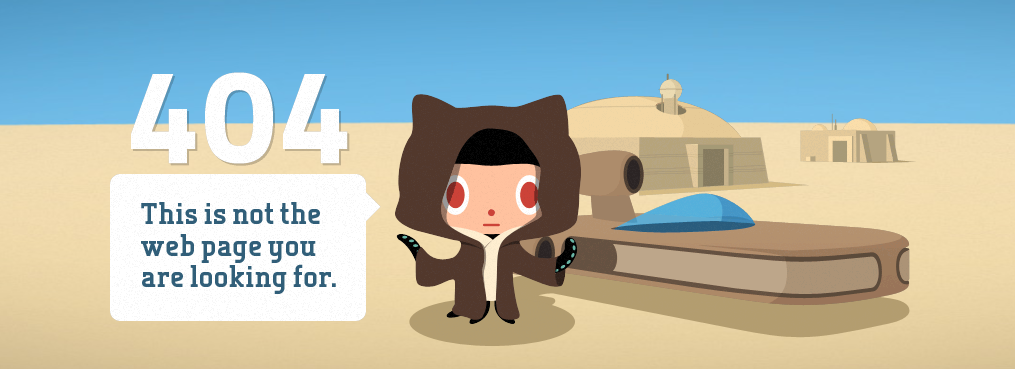
\includegraphics[width=\textwidth]{img/github-404.png}
\caption[Github 404 Error Page]{Github 404 Error Page}
\end{figure}
\noindent
The specific content you tried to reach has been deletet or has been moved by the sites provider. All the links provided are now useless. Every day content gets moved around or is deleted forever. Sometimes its just a silly picture of a cat but mostly its data somebody actually would have needed.\\[0.3cm]
Nevertheless there are several companies already trying to solve this issue by archiving all the data available on the internet. The most well known would be ''Internet Archive'' with its ''Wayback Machine'' Webapplikation. They are using web crawlers to get the data and store them. The User is able to use theWayback Machine to view the webpage back then when the Internet Archive made a snapshot of it \cite{InternetArchive}. By October 2016 they managed to archive 273 billion webpages from over 361 million websites, which resulted in a data size of 15 Petabytes (15'000 Terabytes) \cite{InternetArchiveCount}.

\newpage

\section{Centralization \& Proxy}
Big data hosting companies like Google or Amazon own datacenters worldwide. Developer can buy the service from them to cluster their application data  and distrbute it all over the world. This ensures the availability of your Application even in case of a datacenter outage caused by a natural catastrophe or other technical issues. Those incidents aren't fictions and cost millions if they happen. Latest example, 28.02.2107 the Amazon S3 System located in Northern Virginia gots unavailable. Thousands of webpages and webapplications stopped working. A Amazon technican wantet to remove a small subset of servers. He entered the command wrong and more servers than planned were removed. This led to an 4h outage of the hole Site \cite{AWSOutage}. Estimated cost 150 Million US Dollar \cite{AWSOutageCost}.\\\\
Clustering of data is not standard today. To make your data highly available is cost intensive. To achieve the same level of high availability cost effective without any kind of big service provider like Google is near impossible.\\\\
A second group of big data handlers are the so called CDNs. These Content Delivery Networks host data worldwide and act as a proxy for data requests. Services of these providers are used to bring content closer to the customers to reduce latency and download time.

\section{Privacy \& Consumer Protection}
In these days one of the main concerns of social media platforms are privacy issues and hate messages. Those companies, for example Facebook and Twitter, are facing huge fines in several countries because goverments think they don't do enouth to protect their users. \cite{HateSpeech}. Content shared with a service in the internet, mostly stayes in the internet as its rapidly shared and distributed. If it's out there it's out there forerver. The content itself is hard to locate and remove. The data is adressed with links. The links or URL changes from hoster to hoster. If the affacted user tries to notify the hoster of the data, for example a picture with the intetion to damage the users reputation, it might alread be hosted by several other platforms.

\chapter{Functionality}
\section{How it works}
\subsection{Content Adressing}
Data which is access by HTTP is adressd with its hostname, port, path and the filename.
\begin{exmp}

\end{exmp}
\noindent
IPFS goes a different way. Data added to the global IPFS can be adressed by the hash of its content.

\section{Cryptography}
\section{Versioning}
\section{Storage}
\section{Naming System}

\chapter{Who profits}

\chapter{Future}
The Question is: ''Is there a future for IPFS''?

%https://www.sitepoint.com/http-vs-ipfs-is-peer-to-peer-sharing-the-future-of-the-web/


\begin{thebibliography}{1}
\bibitem{IPFSBasics} \url{https://github.com/ipfs/ipfs}, 24.07.2017
\bibitem{TodaysProblems} \url{https://ipfs.io/}, Sector: The web of tomorrow needs IPFS today, 22.04.2017
\bibitem{InternetArchive} \url{https://en.wikipedia.org/wiki/Internet_Archive}, 22.04.2017
\bibitem{InternetArchiveCount} \url{https://blog.archive.org/2016/10/23/defining-web-pages-web-sites-and-web-captures}, 22.04.2017
\bibitem{AWSOutage} \url{https://aws.amazon.com/message/41926/}, 23.04.2017
\bibitem{AWSOutageCost} \url{http://www.npr.org/sections/thetwo-way/2017/03/03/518322734/amazon-and-the-150-million-typo}, 23.04.2017
\bibitem{HateSpeech} \url{https://www.nytimes.com/2017/03/14/technology/germany-hate-speech-facebook-tech.html?_r=0}, 23.04.2017
\bibitem{HTTPAdressing} \url{https://www.w3.org/Addressing/HTTPAddressing.html}, 23.04.2017 
 
\end{thebibliography}

\printglossaries

\listoffigures
\chapter{RESEARCH}
Research: Merkel DAG, Bittorrent Swarm, Distributed Hash Table, Bittorrent MainlineDHT, multihash, Bitswap

\end{document}